\chapter{Programmazione concorrente}

La programmazione concorrente è l'insieme delle tecniche, metodologie e strumenti per il supporto all'esecuzione di sistemi software da insieme di attività svolte simultaneamente.

Inizialmente implementata attraverso interruzioni (problemi con variabili comuni), oggi la programmazione concorrente è resa più facile dal reale parallelismo reso possibile da sistemi multiprocessore sempre più diffusi.

Le decisioni prese in merito di metodi di suddivisione dei processi e corretta sincronizzazione dipendono da tipo di applicazione e di architettura disponibile.

\section{Tipi di architettura}
\begin{figure}[H]
    \caption{Architettura single processor}
    \centering
    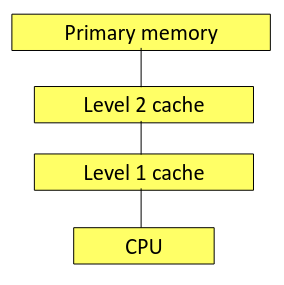
\includegraphics[width=0.45\textwidth]{/home/riccardoob/appunti/sistemi_operativi/images/10.png}
\end{figure}

\subsection{Sistemi multiprocessore}
\begin{figure}[H]
    \caption{Architettura memory multiprocessor}
    \centering
    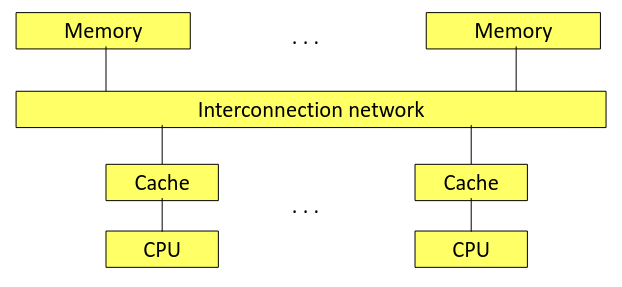
\includegraphics[width=0.6\textwidth]{/home/riccardoob/appunti/sistemi_operativi/images/11.png}
\end{figure}

Due modelli:
\begin{itemize}
    \item \textbf{UMA}: sistemi a multiprocessore con un numero ridotto di processori (da 2 a 30 circa)
    \begin{itemize}
        \item la rete di interconnessione realizzata tramite \textit{memory bus} o \textit{crossbar switch}
        \item Uniform Memory Access: tempo di accesso uniforme a da ogni processore a ogni locazione di memoria, chiamati anche \textbf{SMP} (symmetric multiprocessors).
    \end{itemize}
    \item \textbf{NUMA}: sistemi con un numero elevato di processori (decine o centinaia)
    \begin{itemize}
        \item memoria organizzata gerarchicamente per evitare congestioni sui bus
        \item rete di interconnessione composta da insieme di \textit{switches} e \textit{memorie} strutturato ad albero, distanze variabili dai processori
        \item Non Uniform Memory Access: tempo di accesso non uniforme
    \end{itemize}
\end{itemize}

\subsection{Distributed memory}
\begin{figure}[H]
    \caption{Architettura Multicomputers e Network systems}
    \centering
    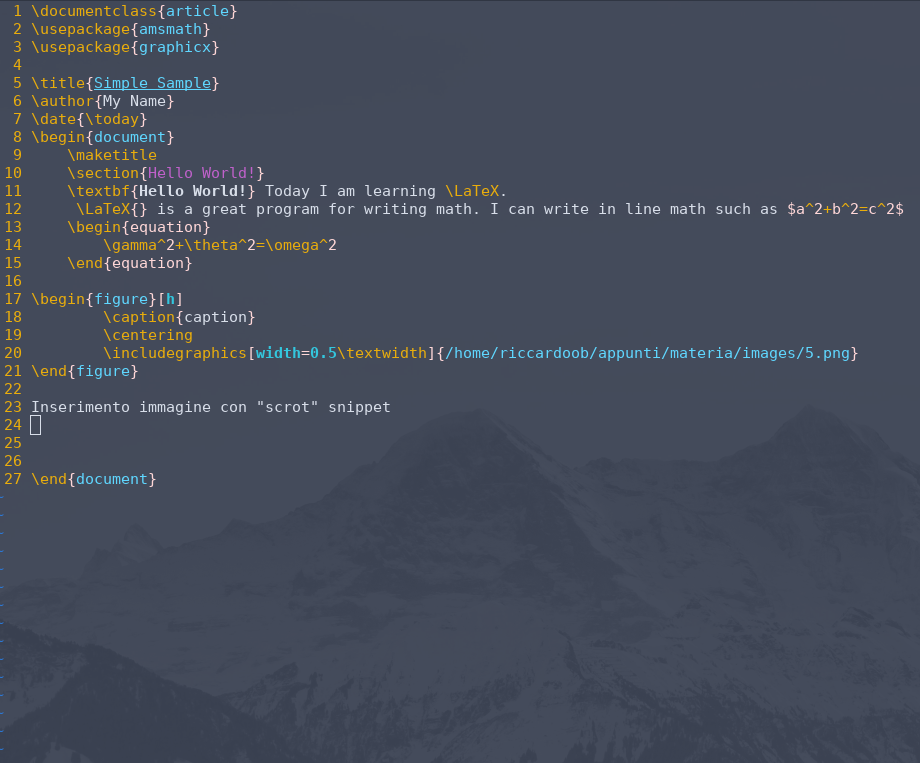
\includegraphics[width=0.6\textwidth]{/home/riccardoob/appunti/sistemi_operativi/images/12.png}
\end{figure}

Due modelli:
\begin{itemize}
    \item \textbf{Multcomputer}: processori e rete fisicamente vicini $\rightarrow$ \textit{tightly coupled machine}, la rete di interconnessione offre un cammine di comunicazione tra i processori ad alta velocità
    \item \textbf{Network systems}: nodi collegati da una rete locale o geografica $\rightarrow$ \textit{loosely coupled systems}.
\end{itemize}

I nodi di un distributed memory system possono essere o singoli processori o shared memory multiprocessor.

\subsection{Classificazione di Flynn}

La tassonomia di Flynn è basata su due concetti:
\begin{itemize}
    \item parallelismo a livello di istruzioni
    \begin{itemize}
        \item \textbf{single instruction stream}: esecuzione di un singolo flusso di istruzioni
        \item \textbf{multiple instruction stream}: esecuzione di più flussi in parallelo
    \end{itemize}
    \item parallelismo a livello di dati:
    \begin{itemize}
        \item \textbf{single data stream}: elaborazione di un singolo flusso sequenziale di dati
        \item \textbf{multiple data stream}: elaborazione di multipli flussi di dati paralleli
    \end{itemize}
\end{itemize}

\begin{figure}[H]
    \caption{Tassonomia di Flynn}
    \centering
    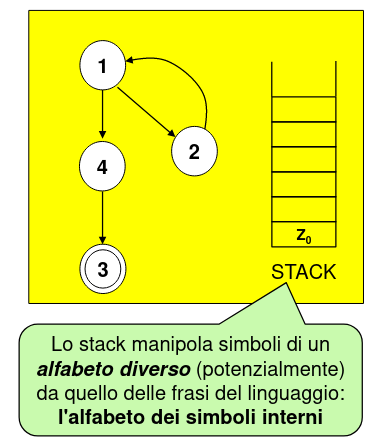
\includegraphics[width=0.7\textwidth]{/home/riccardoob/appunti/sistemi_operativi/images/13.png}
\end{figure}

\section{Applicazioni}

\begin{itemize}
    \item \underline{multithreaded} 
    \begin{itemize}
        \item strutturate come un insieme di processi per far fronte alla \textbf{complessità}, aumentare l'\textbf{efficienza} e per semplificare la programmazione.
        \item i processi possono condividere variabili
        \item esistono più processi che processori (generalmente)
        \item processi schedulati ed eseguiti indipendentemente
    \end{itemize}
    \item \underline{sistemi multitasking/distribuiti} 
    \begin{itemize}
        \item le coponenti dell'applicazione vengono eseguite su nodi collegati tramite opportuni mezzi di interconnessione
        \item comunicazione tramite scambio di messaggi
        \item tipicamente client server
    \end{itemize}
    \item \underline{applicazioni parallele} 
    \begin{itemize}
        \item risolvere un dato problema più velocemente sfruttando il parallelismo disponibile a livello HW
        \item a seconda del modello, istruzioni/thread/processi paralleli interagenti tra di loro
    \end{itemize}
\end{itemize}

\section{Processi non sequenziali e tipi di interazione}

\paragraph{Algoritmo} Procedimenti logico che deve essere eseguite per risolvere un determinato problema.

\paragraph{Programma} Descrizione di un algoritmo mediante un linguaggio, che rende possibile l'esecuzione da parte di un elaboratore.

\paragraph{Processo} Insieme ordinato degli eventi cui da luogo un operatore sotto il controllo di un programma.

\paragraph{Elaboratore} Entità astratta realizzata in hardware e parzialmente in software, in grado di eseguire programmi.

\paragraph{Evento} Esecuzione di una operazione, ogni evento determina una transizione di stato dell'elaboratore.

\subsection{Processo sequenziale}
Sequenza di stato attraverso i quali passa l'elaboratore durante l'esecuzione di un programma.

Un programma può evere più processi associati ad esso, ognuno di questi rappresenta l'esecuzione dello stesso codice con dati di ingresso (possibilmente) diversi.

Un processo può essere rappresentato tramite un grado orientato, detto \underline{grafo di precedenza} del processo, composto da nodi e archi orientati.
Ogni nodo rappresenta un evento corrispondente all'esecuzione di una operazione.

Il grafo di precedenza è a \textbf{ordinamento totale}, ovvero ogni nodo ha un predecessore e un successore.

\subsection{Processo non sequenziale}
Non sempre un processo possiede la proprietà dell'ordinamento totale, molti problemi possono essere risolti più naturalmente tramite processi non sequenziali.

Un \underline{processo non sequenziale} è una successione di eventi seconda una relazione d'ordine parziale.

L'esecuzione di un tale processo richiede un elaboratore in grado di supportare questo tipo di esecuzioni e un linguaggio di  programmazione adatto, non sequenziale.

\paragraph{Elaboratore non sequenziale}
\begin{itemize}
    \item sistemi multielaboratori (a)
    \item sistemi monoelaboratori (b)

\end{itemize}

\begin{figure}[H]
    \centering
    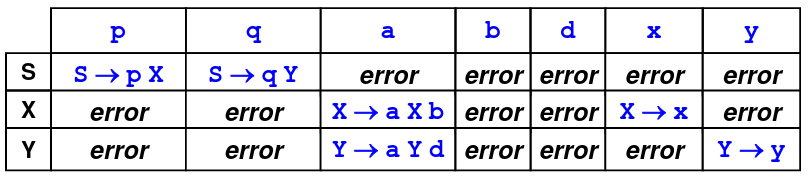
\includegraphics[width=0.8\textwidth]{/home/riccardoob/appunti/sistemi_operativi/images/17.png}
\end{figure}

\paragraph{Linguaggio non sequenziale} consente la descrizione di un insieme di attività concorrenti, sfruttando moduli che possono essere eseguiti in parallelo.

\underline{\textbf{Slide 32-63!!!!!!!!!!!!!!!!!!!!!!!!!!!!!!!!!!!!!!!!!!!!!!!!!!!!!!!!!!!!!!!!!!!!!!!!!!!!!!!!!!!!!!} } 

\section{Proprietà dei programmi}

\paragraph{Traccia dell'esecuzione} Sequenza degli stati attraversati dal sistema di elaborazione drante l'esecuzione del programma.

\paragraph{Stato} Insieme dei valori delle variabili definite nel programma e di quelle implicite.

\paragraph{Programmi sequenziali} Programmi che, su un insieme di dati D si ottiene sempre la stessa traccia.

\paragraph{Pogrammi concorrenti} L'esito dell'esecuzione dipende dalla sequenza cronologica di esecuzione delle istruzioni contenute, lo stesso insieme di dati D può dare una traccia diversa, \underline{non determinismo}.

Verificare che programmi di questo tipo siano corretti non è banale, un semplice debug non garantisce il soddisfacimento di una determinata proprietà.

\subsection{Proprietà dei programmi}

Una proprietà del programma P è un attributo che è sempre vero, data ogni traccia del programma P.

Le proprietà si possono classificare in due categorie:
\begin{itemize}
    \item \textbf{safety properties}
    \item \textbf{liveness properties}
\end{itemize}

\subsubsection{Safety}
É una proprietà che garantisce che durante l'esecuzione di P, non si entrerà \underline{mai} in uno stato "errato".

\subsubsection{Liveness}
É una proprietà che garantisce che durante l'esecuzione di P, \underline{prima o poi} si entrerà inuno stato "corretto".

Nel caso di programmi sequenziali, entrambe le proprietà devono essere realizzate, il programma deve restituire un risultato valido per ogni esecuzione e prima o poi terminare.

Per i programmi concorrenti, si aggiungono anche altri fattori alla completezza della safety e liveness:
\begin{itemize}
    \item Mutua esclusione nell'accesso a risorse (safety): nessun processo accede a una risorsa già occupata da un altro processo contemporaneamente
    \item Assenza di deadlock (safety): per ogni esecuzione non si devono verificare situazioni di blocco
    \item Assenza di starvation (liveness): prima o poi ogni processo potrà accedere akke risorse richieste
\end{itemize}

































































